\special{dvipdfmx:config z 0}
\documentclass[12pt]{article}
\usepackage{graphicx}
\usepackage{float}
\usepackage{amssymb}
\usepackage{amsmath}
\usepackage[UTF8]{ctex}

\author{尹芃淇、刘晖、陈璟、宁白杨}
\title{人机交互论文}
\begin{document}
    \maketitle
    \section{简介}
    \subsection{摘要}
    摘要:随着社会上人口老龄化的问题加深,针对老年人的认知康复训练越来越受到重视。而如何让训练系统在和用户交互的过程中自动分析用户的能力水平,
    从而自动为特定用户设置合适的任务难度,是认知训练目前面临的一大难题。本文主要针对认知训练中的自动难度调节问题,对现有的研究进行了整理归纳,
    总结了在难度调节问题中常用的方法,并对以上方法的优缺点和未来可能的进一步发展进行了分析评价。本文将前人的方法分为两类:基于人工智能的方法和基于生物物理的方法。
    前者通过机器学习和强化学习等多种方式,通过对用户在认知训练中的表现和反应进行建模,从而学习出针对不同用户的难度调节策略,最终实现任务难度个性化;
    后者通过让用户在进行训练任务时佩戴特定的设备,从而采集的用户在特定的生理信号,利用这些生理信号判断用户的实时表现继而调整任务难度。
    \section{研究背景及现状}
        \subsection{人口老龄化}
        我国社会自上世纪末进入老龄化开始,老年人口数量不断增加,老龄化程度持续加深,目前已成为世界上老年人口最多的国家。
        截止 2019 年底,我国 60 周岁以上的人口约 2.54 亿,占总人口的 18.1\%。我国也是世界上老龄化速度最快的国家之一,
        预计到21世纪中叶,我国的老年人口规模将达到 3.8 亿,占总人口的27.9\%。
        
        \subsection{老年认知障碍训练}

        随着我国老年人口数量的快速增长,社会养老、医疗相关的机构面临着越来越大的挑战,因此,社会各界愈发重视老年人的健康问题,不仅包括身体机能老损,也包括认知能力衰退。
        认知障碍疾病是一种以获得性认知功能障碍为核心,导致患者日常生活、工作、学习和社会交往能力衰退,伴或不伴随行为改变的综合征。
        而研究表明认知衰退具有可逆性,依据大脑可塑性和认知储备理论\cite{ref1},
        适当的认知干预会激活神经细胞,增加树突,并形成新的神经通路,使得大脑神经细胞间的信号传导增加\cite{ref2},
        从而延缓甚至逆转认知下降过程。因此基于以上理论设计的对人的认知能力进行的科学测评及系统化训练,
        能够改善认知缺陷和认知减退,提高认知能力\cite{ref3, ref4},改善老年人认知能力衰退的程度。

        \subsection{认知训练现状}

        认知训练是通过对注意力、记忆力、执行能力和语言能力等方面的干预,改善认知功能的过程。
        美国加州大学与芝加哥康复研究所研制康复机器人ARM Guide,通过协助肌肉记忆锻炼对脑卒中病人进行认知康复训练。
        Andriella等人\cite{ref5}提出一种认知机器人系统,提供不同的使用口头和手势交流的鼓励和推荐动作并从所有可用的动作中选择最适合的一个,以减少解决练习所花费的时间。
        Buzzi等人\cite{ref6}创建了一个网络平台,应用行为分析的原则向存在认知障碍的人群提供个性化的学习和培训环境,使用了参与式设计以更好地理解用户需求。
            \section{认知训练难度调节方法}
            认知训练中一个重要的困难点在于如何给被训练者提供难度合适的测试项目,
            针对这一问题业界采取的方法可以分为两个脉络:其一是采取基于生物物理的方法,
            检测其脑电图、行为表现等生物信号,检测其当前状态,以提供合适的测试项目。
            另一脉络是采取基于人工智能的方法,通过被训练者之前的表现检测其当前状态。
        \subsection{生物物理方法}
        生物物理方法的发展从时间上来说,首先从理论方面建立了行为预测心理状态的模型\cite{ref7},
        近年来,寻找了多种能够表征用户心理状态的数据,例如脑电图\cite{ref8}、面部肌电图和电子笔数据等,
        其总体发展趋势是轻便化,追求用户友好,加强沉浸式认知训练,目前出于判断精度与技术成熟水平的考虑,脑电图在研究中更为普遍。
            \subsubsection{}
            \begin{figure}[H]
            	\centering
            	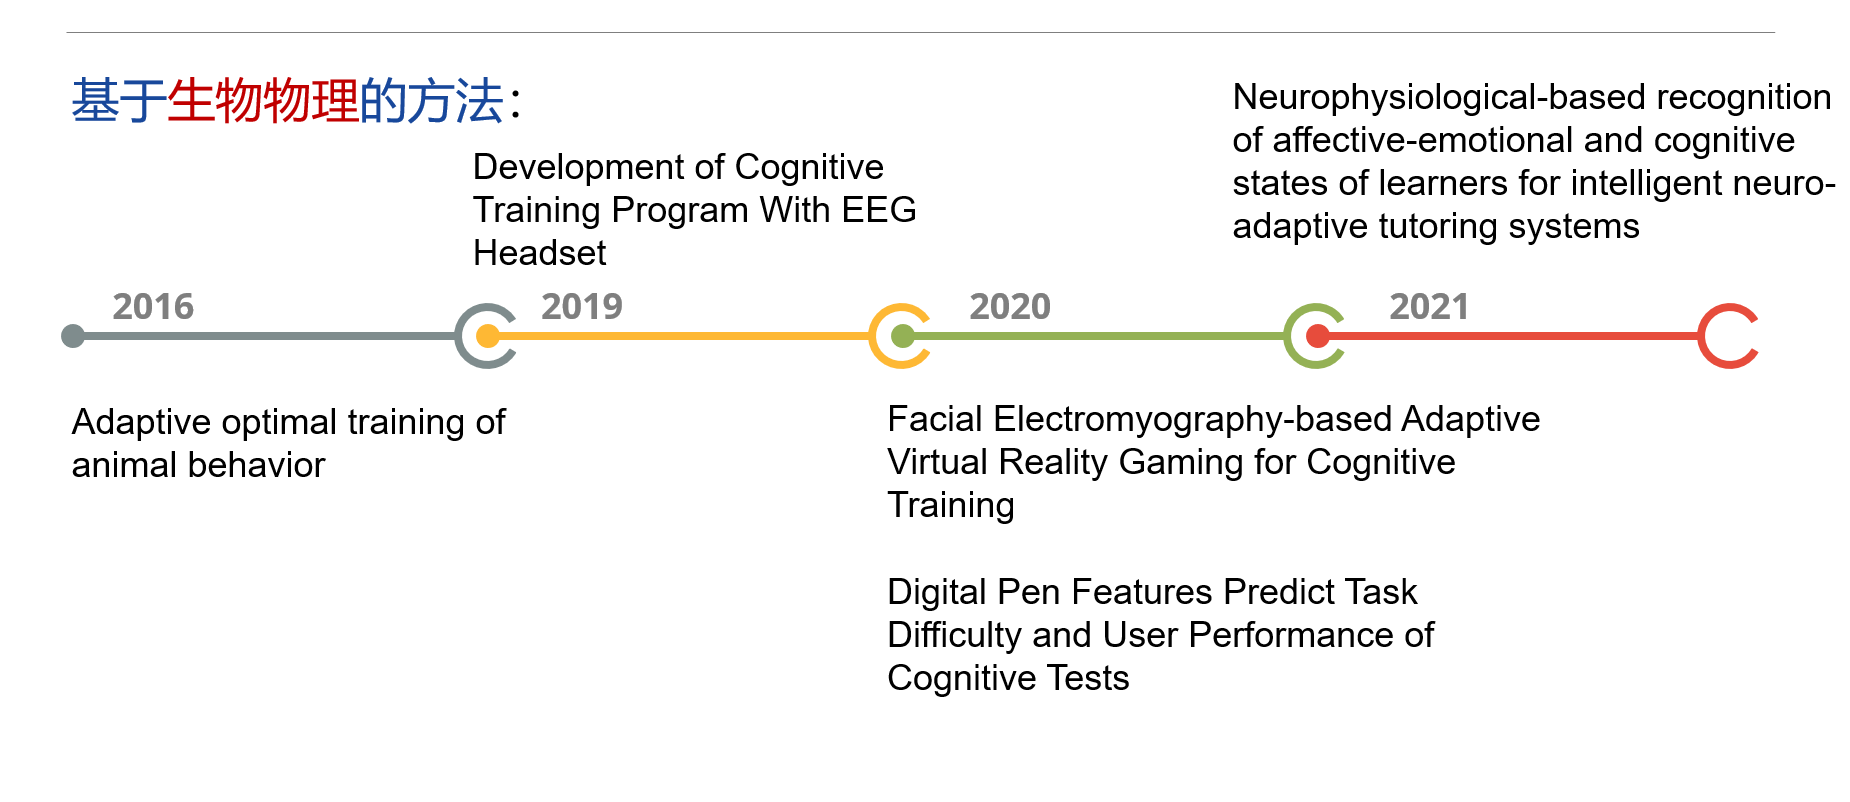
\includegraphics[width=0.8\textwidth]{images/timeline_bio.png}
            	\caption{生物物理方法发展的时间线}
            	\label{fig:label}
            \end{figure}
            首先关注生物物理的方法,这里将查阅到比较核心的论文以时间线的形式在这里列出,
            总结而言,该方法首先是从理论方面建立了行为预测心理状态的模型,
            近年来,寻找了多种能够表征用户心理状态的数据,例如脑电图、面部肌电图和电子笔数据等,
            其总体发展趋势是轻便化,追求用户友好,加强沉浸式认知训练,目前出于判断精度与技术成熟水平的考虑,
            脑电图在研究中更为普遍。接下来,对图中所示的论文内容进行简要阐述。

            \subsubsection{脑电图方法}
            (一) 硬件设置\paragraph{}
            脑电图反映了被训练者的情绪状态,可以被视为被训练者当前对训练难度的反馈。
            据此,ZHIPENG HUANG \cite{ref9}等人提出可以在认知训练中通过采集被训练者的脑电信号来分析被训练者的实时状态,
            进而动态调整训练内容。实验使用可以提供多达16通道的脑电数据的EPOC+耳机作为脑电检测硬件。
            在训练过程中,被训练者在一个虚拟现实环境中,通过键盘和鼠标与环境进行交互完成任务。
            \begin{figure}[H]
            	\centering
            	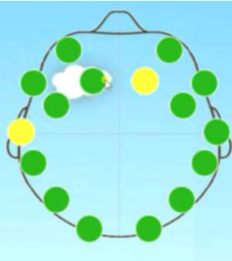
\includegraphics[scale=0.8]{images/brain_distribute.png}
            	\caption{脑电图方法中接收到脑电信号的示意图}
            	\label{fig:label}
            \end{figure}
            (二) 实验设置\paragraph{}
            在实验中,被训练者需要完成反应训练,记忆训练,问题解决训练等。
            在训练过程中,脑电检测硬件会实时采集16通道的脑电数据。
            将该数据作为输入向量分析后,可以得出被训练者当前的情绪状态,
            如“中性”,“焦虑”等。实验将根据被训练者的情绪状态调整训练难度。

            (三) 结果评估与分析\paragraph{}
            实验结果显示,根据脑电图动态调整难度的方法可以带来显著的认知能力提升,
            且比常规训练在提高注意广度和问题解决方面更有效,
            但对反应速度和记忆力没有影响。

            脑电图方法相较人工方法的优势在于能够量化被训练者感知的训练难度,在数据表现上更直观更精准。

            这种方法的缺陷则在于其需要非侵入性的脑电波设备完成检测,对于不同生活习惯的被训练者可能会施加不同程度的外界影响,
            尤其在对老年人进行认知训练时,VR式的显示设备在当前技术条件下可能存在一定的生理负担。
            \begin{figure}[H]
            	\centering
            	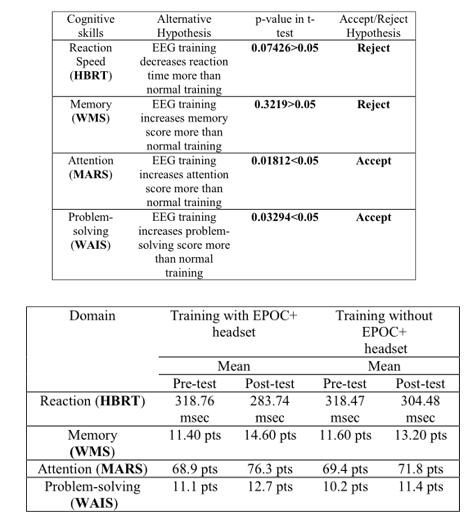
\includegraphics[scale=0.8]{images/brain_data.png}
            	\caption{脑电图方法的实验结果}
            	\label{fig:label}
            \end{figure}

            \subsubsection{面部肌电图方法}
            (一) 硬件设置\paragraph{}
            除了脑电图,面部肌电图同样可以反馈被训练者当前的情绪状态,
            Lorcan Reidy\cite{ref15}等人提出了基于面部肌电图的情感反馈回路。
            \begin{figure}[H]
            	
            	\centering
            	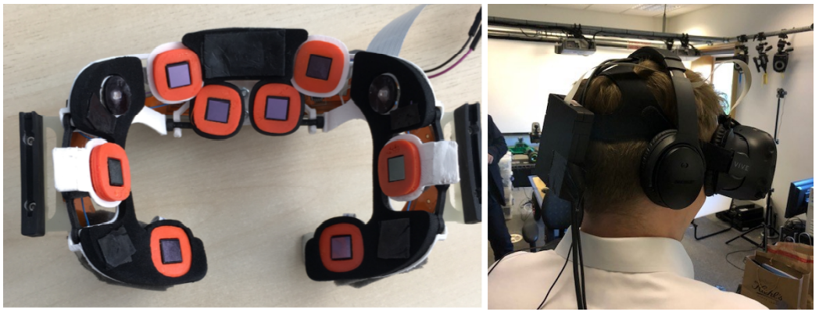
\includegraphics[scale=0.8]{images/Faceteq.png}
            	\caption{面部肌电图方法的硬件基础:配有Faceteq传感器的VR头戴式耳机\cite{ref15}}
            	\label{fig:label}
            \end{figure}
            如图所示,通过让用户佩戴装配有Faceteq传感器的VR头戴式耳机,
            捕捉用户进行认知训练时的实时面部肌肉活动信号,
            采用哈尔小波变换提取数据特征并筛选后通过已有的机器学习模型完成情感分类,
            得出用户当前的情感状态。实验将根据用户的情感状态调节任务难度。

            (二) 实验设置\paragraph{}
            如图所示,实验设计了超市和博物馆两个VR环境和相应的任务来训练用户的记忆力。
            \begin{figure}[H]
            	
            	\centering
            	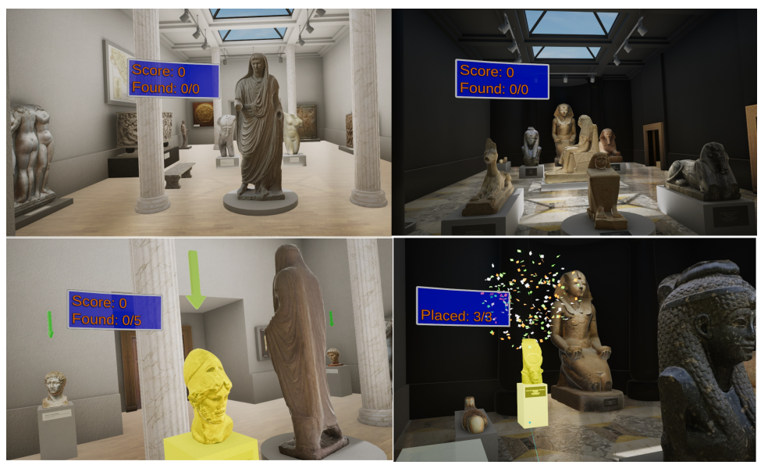
\includegraphics[scale=0.8]{images/VR.png}
            	\caption{VR训练环境:超市和博物馆\cite{ref15}}
            	\label{fig:label}
            \end{figure}
            难度等级根据需要记忆信息的数量分为三个等级。
            从任务的初始点开始,每经过45秒时间间隔记录一次肌电图数据,
            并要求用户通过VR激光笔在屏幕滑块上选择最能描述自己情感状态的选项。
            实验将根据这两者共同判断用户的情感反馈。

            (三) 结果评估与分析\paragraph{}
            实验的效果通过对被训练者的问卷调查得出。
            根据调查结果,加入情感反馈调节之后,
            体验感明显变好,对难度的感受有所降低,
            表明认知训练中用户参与度因为难度提升而降低的问题得到了一定程度的改善。
            此外,对难度提升的感受下降,流动感小幅度提升,总体感受更为积极,
            表明改进后的难度调节模型能够提供较为适宜的难度,
            让用户付出一定的努力并较好地完成任务。

            采用脸部肌电图技术的好处有三点:
            1.相较于其他方法,脸部肌电图技术的数据噪声相对小;
            2.脸部信号能提供较为丰富的交流信息;
            3.解决了基于计算机视觉的面部表情分析在VR的环境下由于设备对面部的遮挡而不适用的问题。

            此外,相较于脑电图技术,根据参与者的反馈,面部传感器并未带来不适感或干扰,对用户更为友好。

            该方法的局限性在于1.目前的测试实验中参与者样本较少,说服力有待增强;
            2.并且脸部肌电图虽适用于VR环境,但在非VR的环境下不一定优于其他方法,因此该方法在其他环境下的优越性有待验证。

            \subsubsection{电子笔信号}
            (一) 硬件设置\paragraph{}
            Barz等人\cite{ref10}的研究认为,任务难度可以作为衡量解决任务所需心理努力的一种标准。
            当使用电子笔进行手写时,采集到的文本和图像数据包含了通过行为表现的生物信号,
            笔端检测到的压力可以体现用户当前的心理努力和情绪状态,如享受或沮丧。
            因此本研究选用学习者用电子笔完成任务时笔端采集得到的数据特征来预测任务的难度和学习者在该任务中的表现。

            (二) 实验设置\paragraph{}
            研究者对儿童进行对照实验,从不同难度的任务中收集电子笔数据,
            并使用不同的学习算法和特征选择策略(支持向量机、梯度增强树)系统地建模了电子笔特征与任务难度和学习者表现的关系。实验中儿童需完成的任务例子如下图所示。

            \begin{figure}[H]
            	
            	\centering
            	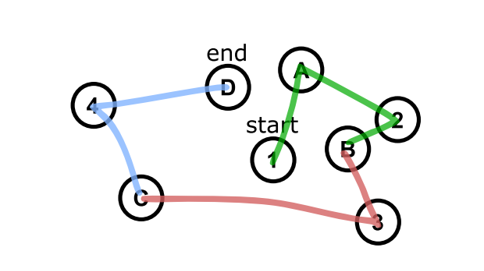
\includegraphics[scale=0.5]{images/digital_pen.png}
            	\caption{将字母和数字按间隔顺序划线连接}
            	\label{fig:label}
            \end{figure}

            (三) 实验结果与分析\paragraph{}
            在实验中,研究者选择了多种不同的特征选择方法,并使用分类算法来区分多个层次的难度。
            实验结果表明,基于电子笔的特征训练可以有效地预测任务内和跨任务的难度水平。
            此外,该模型还可以预测解决一个任务所需的时间。下图展示了实验的具体结果。

            \begin{figure}[H]
        
            	\centering
            	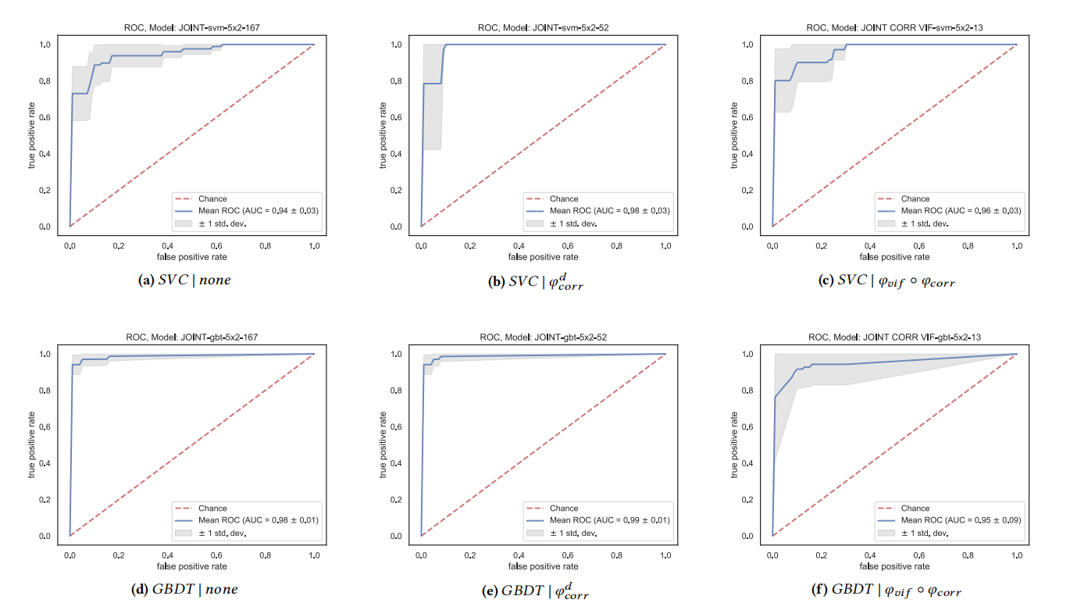
\includegraphics[scale=0.3]{images/pen_result.png}
            	\caption{电子笔调节难度的实验结果}
            	\label{fig:label}
            \end{figure}

            这种方式的优势在于收集人在交互任务时作用在媒介上的生理信号可以反馈用户当前的心理和生理状态,笔端压力是很容易量化的选择。
            但是缺陷是其只在特定训练方式下有效,在用户完成与书写和绘图无关的训练任务时就无法作为采集生理信号的媒介,应用范围较窄。我们认为其他的媒介(如体感交互游戏时的手柄等)也可以承担类似的作用和功能。
            


            
        \subsection{人工智能方法}
        人工智能方法的研究主要围绕机器学习、强化学习和深度强化学习展开,通常是多种方法的结合运用,总体上来说多采用机器学习和深度学习的方式对用户进行分类,再借助强化学习方法利用新数据更新迭代现有模型,探索对用户的个性化任务难度。
        \subsubsection{}
        \begin{figure}[H]
            	
            \centering
            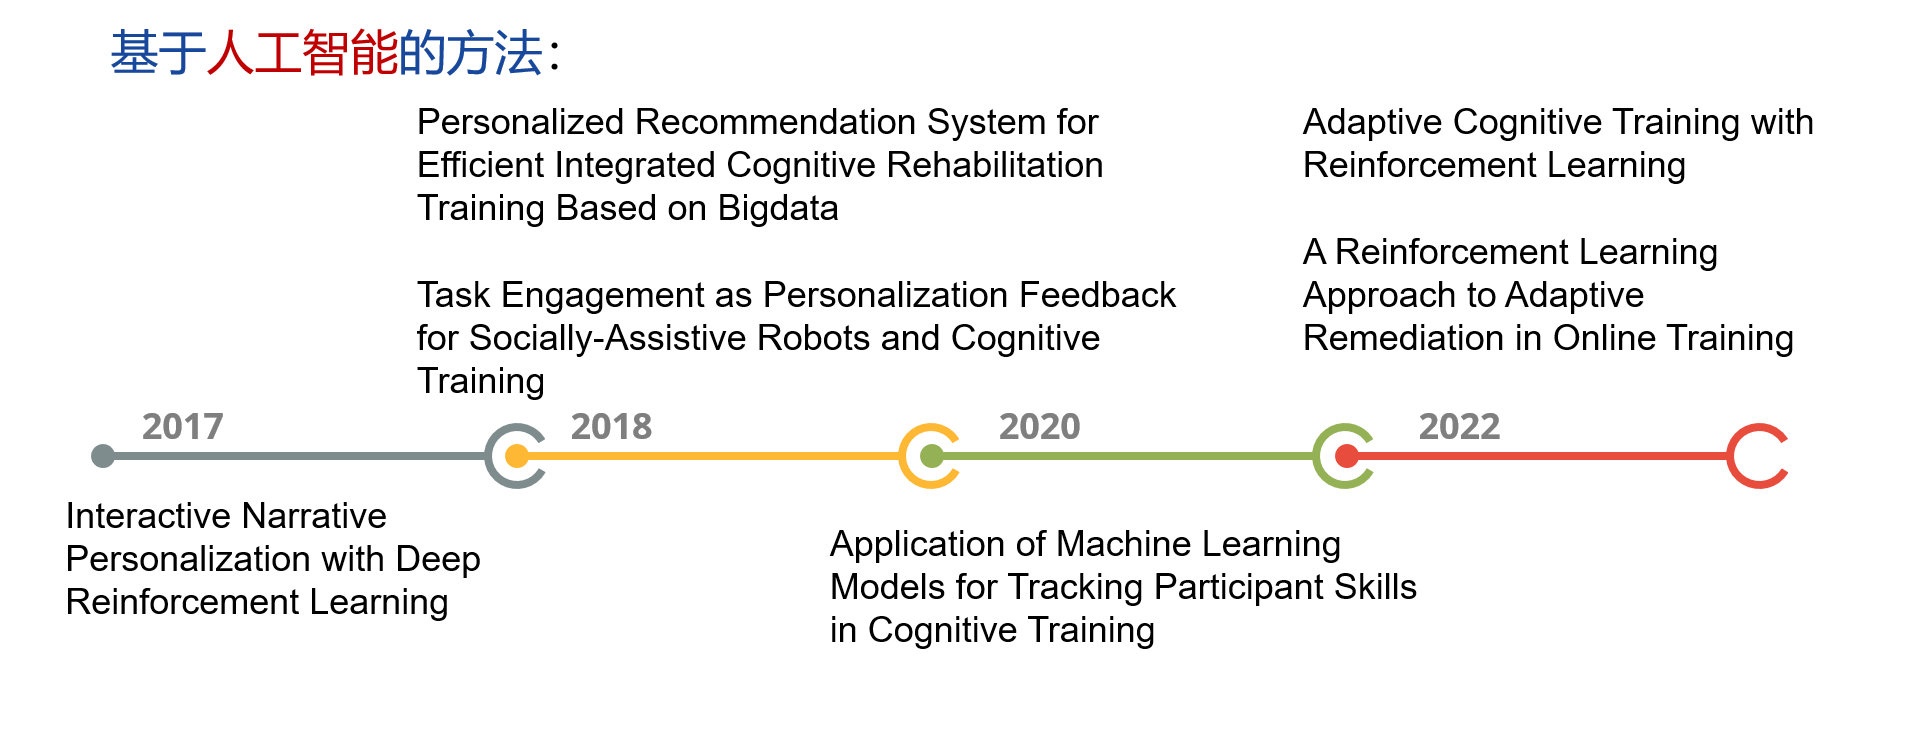
\includegraphics[width=0.8\textwidth]{images/timeline_AI.png}
            \caption{人工智能方法发展的时间线}
            \label{fig:label}
        \end{figure}
        下面是人工智能方法的脉络,本文将比较核心的论文以时间线的形式列出,
        通过调研发现,该方向的研究主要围绕机器学习、强化学习和深度强化学习展开,
        通常是多种方法的结合运用,总体上来说多采用机器学习和深度学习的方式对用户进行分类,
        再借助强化学习方法利用新数据更新迭代现有模型,探索对用户的个性化任务难度。
        以下将对列出的论文进行简要阐述。

        \subsubsection{机器学习}
            (一) 实验设置\paragraph{}
            Sanjana Sandeep\cite{ref16}等人指出,认知训练中现有的难度自适应算法大多只参考用户最近几次的任务表现,
            而贝叶斯方法和深度学习模型可以对用户在较长时间内的、多轮次的训练轨迹进行建模并预测用户下一次的任务表现,
            从而据此设置合适的任务难度。
            实验召集了两组参与者,使其完成三种锻炼工作记忆的认知训练任务,全程采集被训练者在任务中的数据表现,
            并选用隐马尔科夫模型、卡尔曼滤波模型和LSTM模型三种方法对其建模。

            (二) 实验结果与分析\paragraph{}
            实验结果表明,三种方法都能合理预测适宜的难度,
            其中隐马尔科夫模型对用户在特定难度下的表现预测最为准确,
            因此性能最佳。实验结果证明了机器学习方法在任务难度个性化上有较大的潜力。

            我们认为机器学习方法的优势在于能够综合长期训练表现以及能够处理高维数据,
            并且仅需记录用户任务表现训练得到,对传感器无要求。
            但缺点在于预先需要大量的训练数据,并且相比起传感器实时监测调节的方法,
            耗时相对长。

            \subsubsection{大数据与机器学习}
            (一) 实验设置\paragraph{}
            Jeong Joon Kim\cite{ref11}等人指出,简单的基于计算机的认知康复重复训练难以帮助患者恢复认知功能,若选择在医院陪伴治疗会造成资金、空间和时间上的负担。
            因此开发了基于大数据的高效综合认知康复训练个性化推荐系统,该系统具有复杂的难度等级结构,并根据平均响应时间和游戏训练结果通过算法自动调整难度等级。
            希望帮助老年人发现轻度认知障碍的初始阶段,并提供个性化训练方式。

            其整体架构如图所示,分为综合管理组件、大数据处理组件和个性化推荐组件三个部分。
            \begin{figure}[H]
            	
            	\centering
            	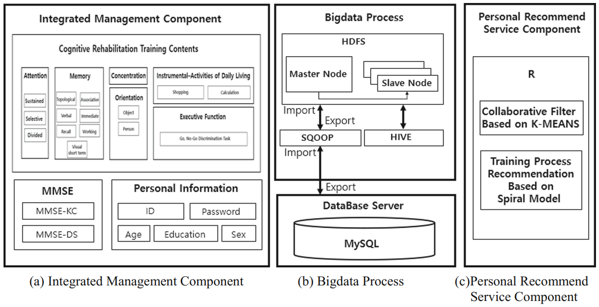
\includegraphics[scale=0.7]{images/Overall_architecture.png}
            	\caption{基于大数据的认知训练个性化推荐系统整体架构}
            	\label{fig:label}
            \end{figure}

            综合管理组件:将提前收集的难度分级训练内容、认知等级测试结果(训练时间、反应次数、准确度和反应时间)和个人信息保存在MySQL数据库服务器。
 
            大数据处理组件:利用SQOOP将数据库信息导入Hadoop HDFS(分布式文件系统)进行保存,其数据由HIVE进行查询和处理。

            个人推荐服务组件:利用K-MEANS进行用户聚类,利用相似的个人信息和具有认知康复内容结果(训练时间、反应次数、准确度和反应时间)的患者,预测新患者或信息不多患者的认知能力和相关数据,并提出如图所示的基于流理论和分形模型的螺旋式训练模型,让患者在接受挑战与精神放松之间切换,提高学习效率。
            \begin{figure}[H]
            	
            	\centering
            	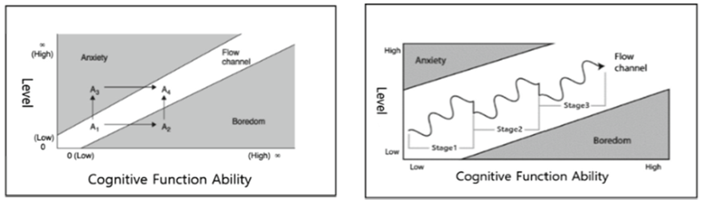
\includegraphics[scale=0.7]{images/flow_theory.png}
            	\caption{螺旋训练模型参考的流理论和分形模式}
            	\label{fig:label}
            \end{figure}
            
            


            (二) 实验结果与分析\paragraph{}
            文中表示搭建的基于大数据的模型能够通过聚类的方式对新患者的认知能力进行快速分类,
            并选择适当的任务设置难度范围,再基于提出的螺旋式训练模型,
            能够让病人持续的跟随训练。

            我们认为本系统为患者认知能力水平预测提供了一个基于大数据的分类思路,
            但由于缺乏后续的实验数据调查,其分类准确度没有明确指出,
            并且系统缺乏一定的训练结果反馈,可能导致分类效果不佳,
            可在后续进行性能上的优化。不过,文中提出的螺旋训练模型值得借鉴,
            其不仅在每一阶段实现训练难度上的递进,
            还能在阶段内通过难度的细微调节来调动患者的积极性。






            \subsubsection{强化学习}
            (一) 实验设置\paragraph{}
            FLORIANO\cite{ref12}等人提出,可以使用强化学习的方法,通过提取训练中被训练者的表现数据作为输入来改变模型。
            为了防止被训练者在过于偏离正确值的难度标准下丧失训练兴趣,
            模型的初始化值在人类训练专家的建议下设定。

            实验分为两个阶段:第一个阶段使用所有被训练者的数据对模型进行训练,
            以达到在人群上较好的泛化性;第二个阶段对于每个训练者单独训练模型,
            以达到对个人更加精准调整难度的效果。
            \begin{figure}[H]
            	
            	\centering
            	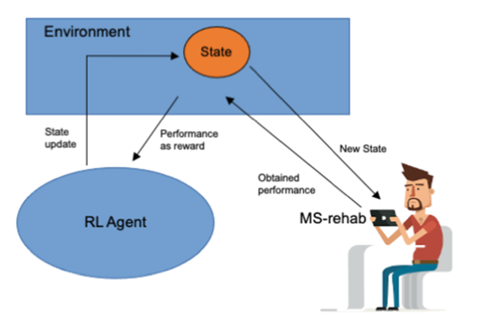
\includegraphics[scale=0.7]{images/RL_stage.png}
            	\caption{强化学习的基本流程}
            	\label{fig:label}
            \end{figure}
            (二) 实验结果与分析\paragraph{}
            实验结果表明,在大学生的认知训练过程中使用强化学习这种有效的类别策略是可行的。
            结果显示经过这种方法的认知训练后被训练者的神经心理学指标PASAT出现显著改善,
            且与使用由认知康复专家设计的指导训练过程的政策所获得的改善相比具有更大的相关性。

            通过允许强化学习在训练过程中使用为个体进一步学习定制的策略,
            为学生学习的类别策略可以进一步得到改善。
            虽然被训练者在PASAT中获得的结果没有继续明显提升,
            但该策略能够帮助他们在更短的时间和更少的练习中获得同等的结果。

            通过强化学习,我们得到了一种无需外置传感设备便能动态调整训练难度的方法,
            且这种方法可以实现高度的个性化。但是强化学习对输入的数据有大量需求
            ,如何保证被训练者在模型的学习期间的热情是一个亟待解决的问题。此外,
            针对每个个体单独训练模型虽然可以提升训练效果,
            但也造成了训练成本的大幅上升。

            \subsubsection{深度强化学习}
            (一) 实验设置\paragraph{}
            Pengcheng Wang\cite{ref13}等人提出,线性的强化学习在动作空间和样本空间都有明显的局限性,
            然而比较复杂的、更加接近实际情况的任务则往往有着很大的状态空间和连续的动作空间。
            对此他们提出可以使用深度强化学习的方法,利用深度学习拟合玩家当前状态,
            再通过强化学习得到相应动作,以适应任务难度。

            本研究以教育性互动叙事游戏CRYSTAL ISLAND为背景,玩家通过虚拟阅读和与NPC互动获取线索,根据交互时的用户选择,采用不同的方式进行剧情推进。以学习收益(NLG)作为游戏指标,当触发适应性事件时,机器根据当前玩家已获得的线索或测试成绩,提供不同详细程度的线索,使玩家收获较高游戏的游戏满意度和学习收益。
            
            其整体框架如图所示,分为数据层,玩家模拟层,强化学习层和适应性叙事层四层结构。
            收集现实玩家数据和学习收益调查结果,并将其随机分为训练集和测试集。
            基于LSTM模型进行玩家模拟,为深度强化学习训练提供大量数据支持,再构建的深度强化学习层进行策略优化,最后利用适应性叙事层进行评估。
            \begin{figure}[H]
            	
            	\centering
            	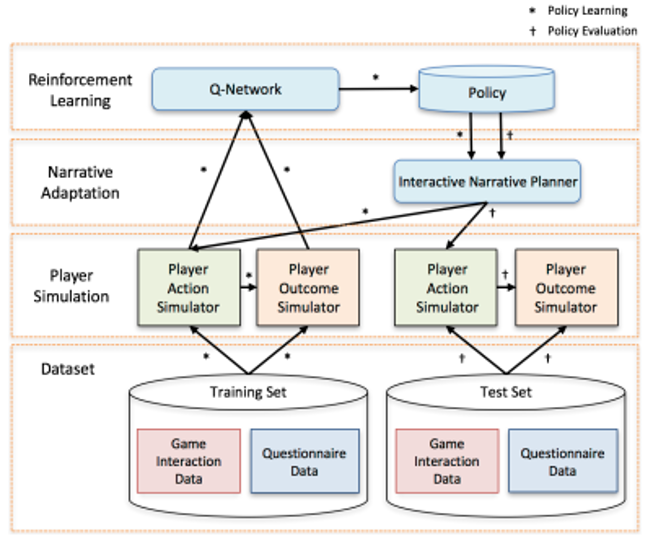
\includegraphics[scale=0.5]{images/RL_architecture.png}
            	\caption{深度强化学习系统架构}
            	\label{fig:label}
            \end{figure}

            (二) 实验结果与分析\paragraph{}
            通过对比采用线性强化模型和不同Q-network的强化模型进行交互得到的收敛策略值,如图所示,表明使用Q网络可以提高非线性复杂玩家互动模式的能力,
            合理配置的Q网络RL互动叙事规划器可以显著优于基于线性RL的互动叙事规划器,并且证实了LSTM加入Q网络的有效性,适用于需要长期记忆的特殊情况。
            \begin{figure}[H]
            	
            	\centering
            	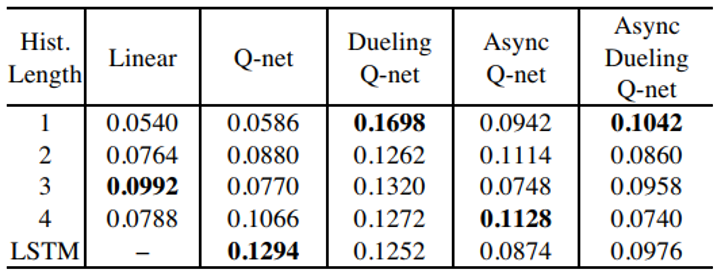
\includegraphics[scale=0.6]{images/policy_value.png}
            	\caption{与玩家进行10000次互动后优化得到的评估策略值}
            	\label{fig:label}
            \end{figure}

            该方法的优势在于算法通用性强,是一种端到端的处理方式,可为监督学习产生大量的样本。
            但缺点在于需要大量训练数据(在本文中由玩家模拟层提供),训练时间长,且算法不一定收敛,需要仔细调参。

            \subsubsection{强化学习与马尔科夫决策}
            (一) 实验设置\paragraph{}
            Spain等人\cite{ref14}的研究选择了一个现有的适应性训练课程,让学习者完成课程后记录并分析了前试、后试、调查和学习者的互动日志数据。课程形式如下图所示。

            \begin{figure}[H]
            	
            	\centering
            	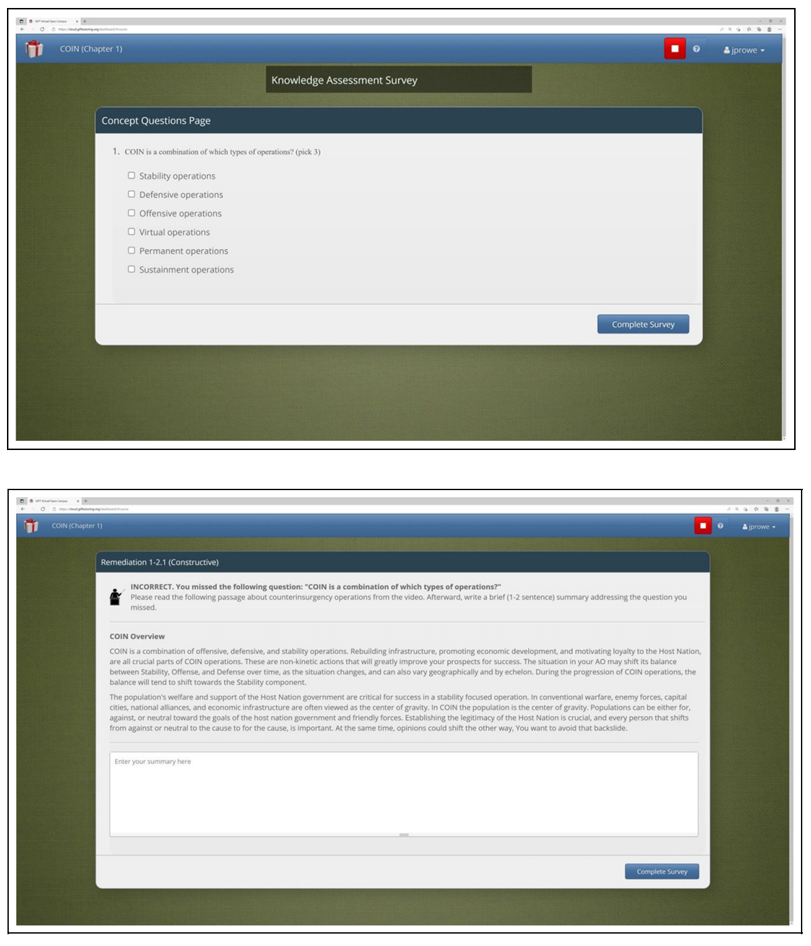
\includegraphics[scale=0.8]{images/Markov_game.png}
            	\caption{学习者参与的课程}
            	\label{fig:label}
            \end{figure}

            在课程中,学习者被提供了反馈和补救内容引发不同程度的认知参与。
            然后利用这些数据将教程计划建模为一个情景任务,其中每个学生日志对应一个强化学习事件,
            基于马尔科夫决策过程创建一套利用强化学习的教程规划策略,根据学习者交互日志数据进行训练,
            可用于在适应性教学系统中为学习者提供适应性补救。

            (二) 实验结果与分析\paragraph{}
            研究归纳了八种不同的策略,对应于四种交替状态表征和两种奖励模型的不同组合。
            实验结果表明,学习者通过教程规划的补救帮助下纠正了导致回答错误的因素。
            同时,在几种补救等级上,建设性补救是最高的,主动补救的优先级始终高于被动补救,
            而被动补救高于不补救,这与课程中逐步淡化脚手架的教学目标一致。
            教程规划所选择的补救方式取决于学生在课程中的进度、学生的先验知识和他们已经获得补救的次数。
            实验的具体结果如下图所示。

            \begin{figure}[H]
            	
            	\centering
            	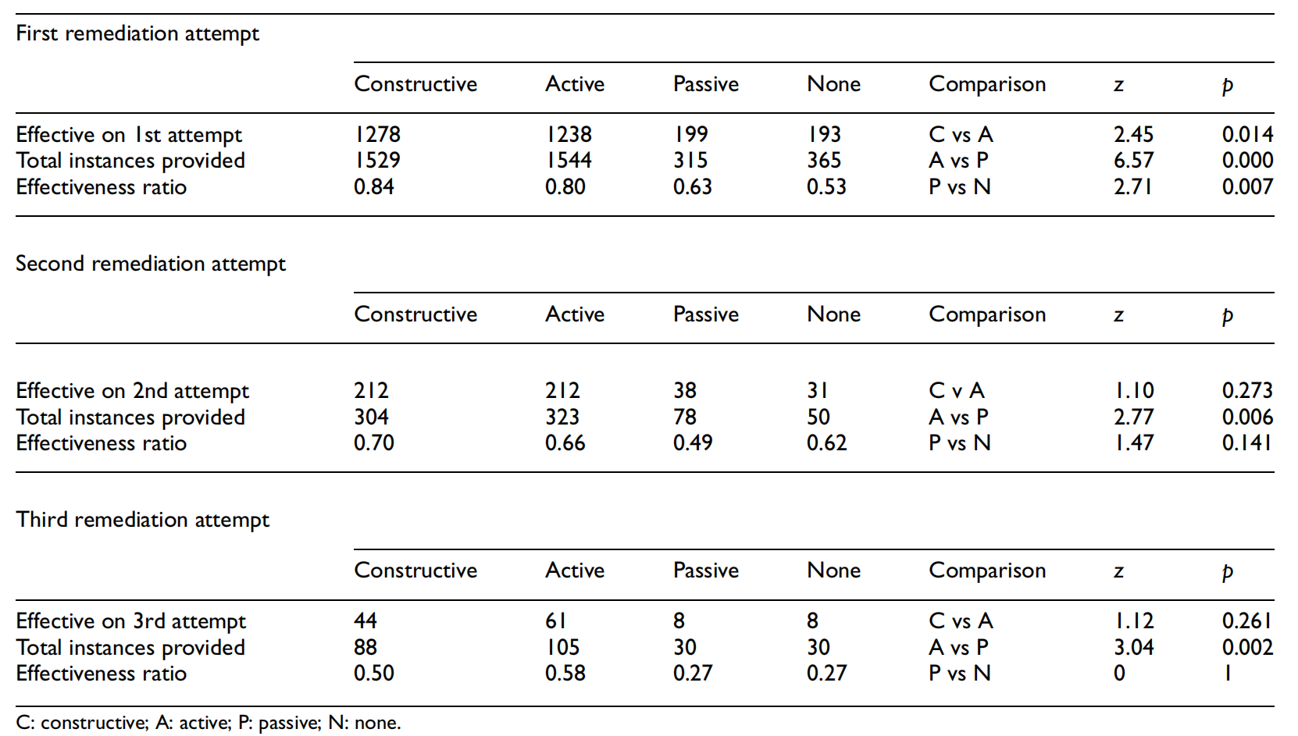
\includegraphics[scale=0.25]{images/Markov_result.png}
            	\caption{马尔科夫决策下的教程规划效果}
            	\label{fig:label}
            \end{figure}

            这种方法的优势在于引入了马尔科夫决策,对学习者状态和补救方式建立了完备的脚手架体系。但它同样具有强化学习的普遍问题,即需要大量的训练数据。
            此外,在这项研究中学习者的先验知识会对实验结果产生影响,
            而先验知识的获得是基于学习者对现有的一个训练课程的完成情况,
            这就意味着对于新的学习者无法在不完成该训练课程直接使用教程规划的情况下获得其先验知识。

            \subsubsection{用户聚类与强化学习}
            (一) 实验设置\paragraph{}
            Konstantinos Tsiakas\cite{ref17}等人提出,难度调节不仅要根据用户在不同难度任务下的得分,
            还要参考用户的脑部状态——用户参与度。因此作者提出了一个交互式强化学习框架,综合考虑用户得分和用户参与度,共同任务难度个性化调节。
            如图所示,
            \begin{figure}[H]
            	
            	\centering
            	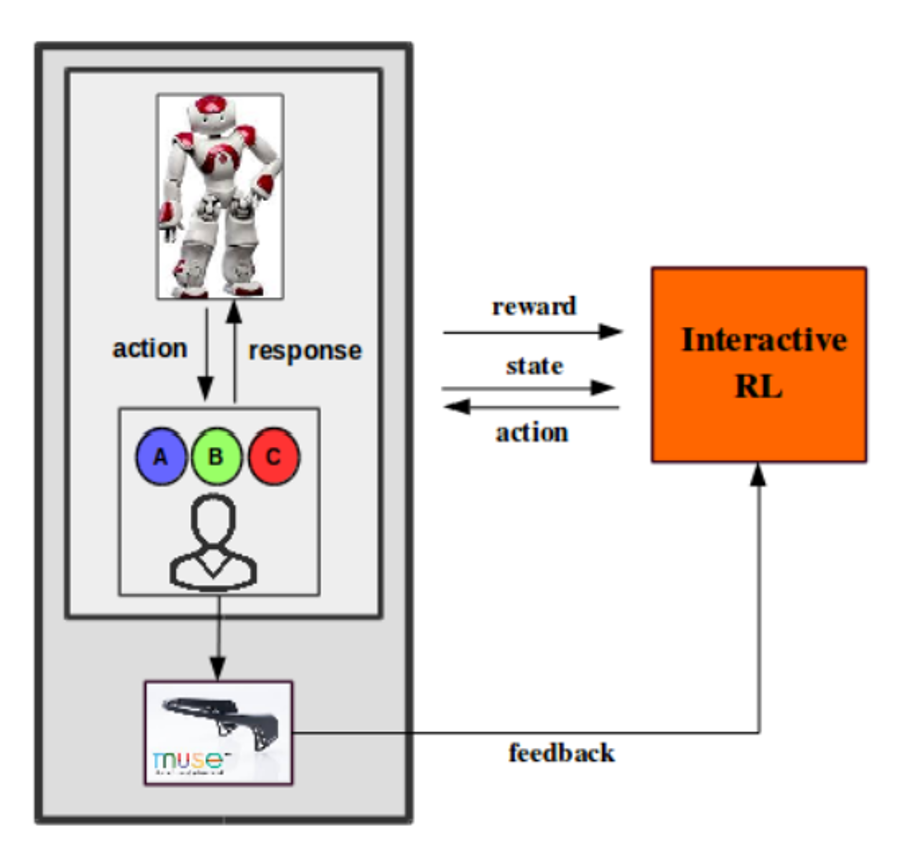
\includegraphics[scale=0.8]{images/RL_Frame.png}
            	\caption{强化学习系统框架\cite{ref17}}
            	\label{fig:label}
            \end{figure}
            它包括物理部分和计算部分,用户进行认知训练时,系统会追踪当前的任务难度、机器人的反馈、用户的任务表现以及通过EEG测量到的任务参与度(task engagement),然后系统通过这些信息调节自身状态。
            在这个过程中,机器人逐渐学习出有效策略,学习根据机器人的反馈和当前状态调节任务难度。
            \begin{figure}[H]
            	
            	\centering
            	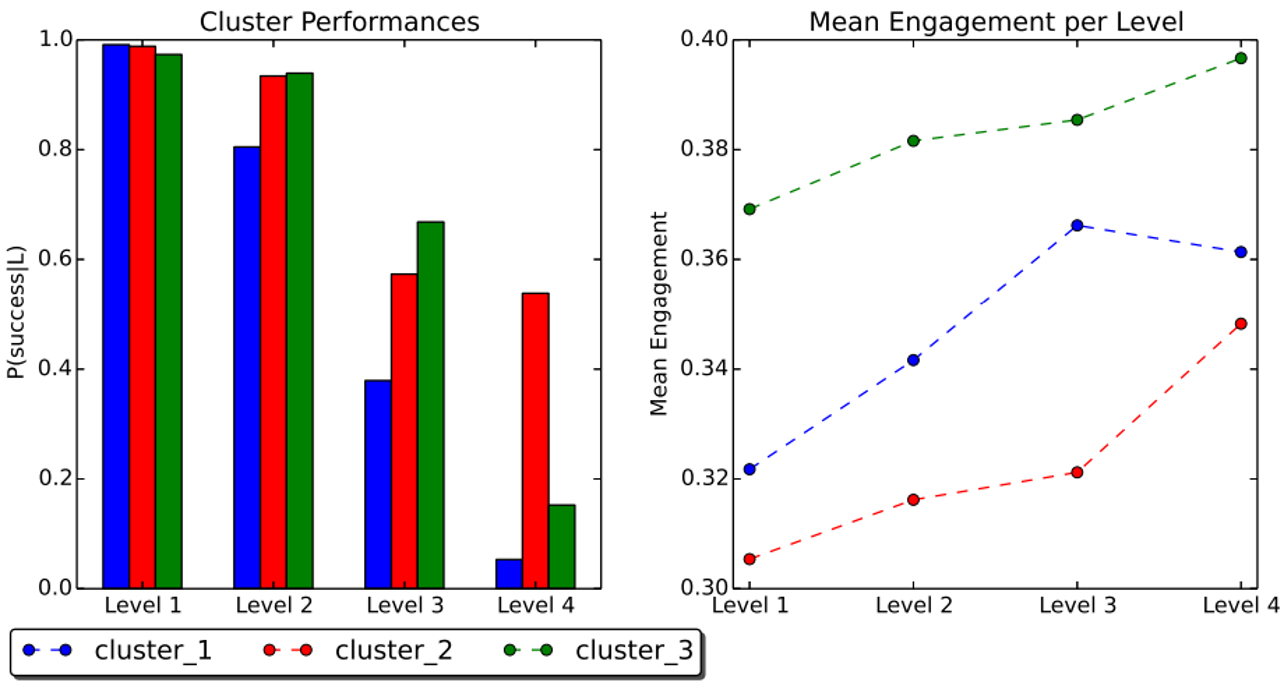
\includegraphics[scale=0.6]{images/user_model.png}
            	\caption{用户聚类\cite{ref17}}
            	\label{fig:label}
            \end{figure}
            在获得上述数据之后,对用户的数据采用k-means聚类,结果如图所示,将用户分成三类,同一类用户可看作是具有相似的水平表现。
            然后通过强化学习,得到针对不同种类用户的最优机器策略。

            (二) 实验结果与分析\paragraph{}
            实验结果显示,在引入用户参与度之后,经过强化学习的训练收敛到最佳策略,
            两种集成用户参与度的方法(调整reward和Q-augmentation)都能给用户的任务表现和任务参与度带来提升,
            都高于仅仅引入任务表现的情况。

            这种方法在思路上较为完备,通过构建一个交互式框架,综合考虑得分和脑部状态,
            学习得到合适的难度策略。但在实际用途上有较为明显的局限性。
            首先,强化学习对大量训练数据的需求导致系统无法在初步交互中快速建立起策略。
            其次,由于样本数量和归类方法的限制,对用户的归类不全面,无法考虑少数个例。
            但本文在宏观框架上为后来的研究提供了较好的借鉴。

            \subsubsection{对主流方法的思考:生物物理信号直接分析}
            生物物理信号分析可以通过传感器直接地反映训练者当下的神经或肌肉活动。

            并且传感器信号具有实时性,可以即刻反映用户某处状态的变化,能让系统快速获得用户反馈并即时根据用户的状态改变策略。

            目前现存的信号来源多种多样,包括采集脑部信号的脑电图、采集面部肌肉信号的肌电图以及电子笔压力等相对间接的物理信号等,
            它们都能一定程度上反映用户的状态变化,并且目前的研究基本只涉及其中一种,未来的研究可以尝试几种信号联合测量用户状态的方法。

            但是,传感器设备反映的是最底层的物理信号,与顶层的意识之间有着复杂的映射关系,将信号与意识关联需要一定的解码。
            例如,在脑电图方法中,从eeg耳机中得到的数据仅能表述被训练者的简单情绪状态,
            例如“平静”和“焦虑”,而无法足够精准量化地反映出对于当前训练者的训练难度。若目标为精准控制训练难度,这种程度的信号精度尚且不够。

            除此之外,为了进行信号采集需要更复杂的设备,这使得生物物理信号分析更为困难。

            并且部分设备可能给用户带来干扰或引起用户的不适反应,比如VR设备可能给部分用户造成晕眩,给戴眼镜的用户造成压迫感等。

            除此之外,部分传感器信号存在较大噪声干扰,因此给信号类型的选择以及去噪工作带来困难。
            
            \subsubsection{人工智能间接分析}
            人工智能方法对传感器设备无要求,仅需训练模型的算力,并且相对于传统难度调节算法具有处理高维数据的能力,
            在认知训练的应用上有较大的发展潜力。

            机器学习或强化学习的方式可以通过训练者的过往表现较好地预测当前训练者适合的训练难度,
            例如贝叶斯方法和深度学习模型可以对用户在较长时间内的、多轮次的训练轨迹进行建模并预测用户下一次的任务表现,从而设置合适的难度。

            但是,训练模型需要大量的数据,并且实现模型预测需要较多的用户数据,因此系统难以在和用户的初步交互中快速建立起策略。
            
            当训练任务种类较多时,进行跨任务的难度调节精度会下降,而如果进行联合训练则成本会提升。
            此外,由于训练者有较大的个体差异性,要准确预测特定个体的适合难度需要对每个训练者的数据都分别进行学习。
            例如在强化学习方法中,作者在使用20位志愿者的数据对神经网络模型进行训练后,
            又使用每位志愿者的数据单独对神经网络进行了训练,这使得模型在针对个人的难度调整能力上更加精准
            ,但是泛化性下降。这使得每个模型在投入个人使用前需要被训练者的配合进行fine-tune,增大了时间成本,对被训练者提出了一定的挑战。
            






    \section{总结与展望}
    \subsection{总结}
    本文的研究是以老年人的认知神经系统的康复训练为中心的。
    在康复训练中,随着用户的训练进程设置和调整符合用户能力的任务难度可以让用户在交互过程中获得符合自身能力的训练,
    以最优化训练过程和训练效果。
    
    为了给用户提供难度合适的训练项目,目前主流的方法第一种是基于人工智能的方法,
    包括机器学习和强化学习等多种方式,通过对用户过往的表现建模来实现任务难度个性化;
    第二种是基于生物物理的方法,采集的用户生理信号包括脑电信号、面部肌肉信号、手写笔触信号等,
    利用这些生理信号判断用户的实时表现继而调整任务难度。
    人机交互研究是对人和计算机的两位一体的研究,随着对人脑与认知的研究的进一步深入和神经网络在计算机领域日益重要的作用,未来基于认知科学、神经生理学和神经科学研究的转化方法将成为认知康复有效治疗发展的有前途的未来方向。



    \subsection{展望}
    人机交互研究是对人和计算机的两位一体的研究,
    随着对人脑与认知的研究的进一步深入和神经网络在计算机领域日益重要的作用,
    未来基于人机交互、认知科学、神经生理学和神经科学研究的转化方法将成为认知康复有效治疗发展的有前途的未来方向。
    经过我们调研总结,未来的认知训练模式将具有以下几个特性:

    1.精准化,个性化,具体化。
    认知训练应当做到为每个个体,每种不同的认知障碍,
    乃至同一个体不同的情绪状态做出区分,在细分领域达成更好效果。

    2.便捷化,实用化。由于需要认知训练人群的特殊性,
    训练的方式应当是易于被接受且无侵入性设备的,
    例如电子笔方法比起面部肌电图方法更加易于被接受且能够被更加方便地部署在使用者日常生活中。
    为了达成这一目的,未来的认知训练方法可能采取类人型机器人辅助训练的方法,
    这样可以方便地增加被训练者的接受度。

    由以上两点我们提出一种新颖的认知训练模式猜想:家庭化机器人训练方法。
    这种方法采取类人型机器人作为与被训练者的沟通终端,从而增加被训练者的接受度,
    使用上文中阐述的深度强化学习构建训练难度自适应调整模块,
    以做到为被训练者特异性地提供训练内容,增强训练效果。

    
    \begin{thebibliography}{99}  

        \bibitem{ref1}Rozzini L, Costardi D, Chilovi BV, et al. Efficacy of cognitive rehabilitation in patients with mild cognitive impairment treated with cholinesterase inhibitors [J]. Int J Geriatr Psychiatry,2007,22(4):356-360.
        \bibitem{ref2}Li BY, He NY, Qiao Y, et al. Computerized cognitive training for Chinese mild cognitive impairment patients: A neuropsychological and fMRI study [J]. Neuroimage Clin,2019,22:101691.
        \bibitem{ref3}申婉丽,张舒涵,黄小璐,魏雷,何清华.线上认知训练的研究现状与训练效果[J]. 心理技术与应用,2019,7(11):671-682.
        \bibitem{ref4}Lovden M, Backman L, Lindenberger U,Schaefer S,Schmiedek F. A theoretical framework for the study of adult cognitive plasticity[J]. Psychological Bulletin, 2010. 136 (4), 659-676.
        \bibitem{ref5}Andriella, A., Torras, C.,  Alenyà, G. (2020). Cognitive System Framework for Brain-Training Exercise Based on Human-Robot Interaction. Cognitive Computation, 1–18.
        \bibitem{ref6}Buzzi, M. C., Buzzi, M., Perrone, E., Senette, C. (2019). Personalized technology-enhanced training for people with cognitive impairment. Universal Access in the Information Society, 1–17. 
        \bibitem{ref7}Bak, J. H., Choi, J. Y., Akrami, A., Witten, I.,  Pillow, J. W. (2016). Adaptive optimal training of animal behavior. Advances in neural information processing systems, 29.
        \bibitem{ref8}Lingelbach, K., Gado, S.,  Bauer, W. (2021). Neuro-adaptive tutoring systems. 
        \bibitem{ref9}Huang Z, Javaid A, Devabhaktuni V K, et al. Development of cognitive training program with EEG headset[J]. IEEE Access, 2019, 7: 126191-126200.
        \bibitem{ref10}Barz, M., Altmeyer, K., Malone, S., Lauer, L., Sonntag, D. (2020). Digital Pen Features Predict Task Difficulty and User Performance of Cognitive Tests. Proceedings of the 28th ACM Conference on User Modeling, Adaptation and Personalization. 
        \bibitem{ref11}Kim, J., Kim, Y., Lee, H., Lee, S.,  Chung, S. (2018). Personalized Recommendation System for Efficient Integrated Cognitive Rehabilitation Training Based on Bigdata. HCI.
        \bibitem{ref12}Zini F, Le Piane F, Gaspari M. Adaptive Cognitive Training with Reinforcement Learning[J]. ACM Transactions on Interactive Intelligent Systems (TiiS), 2022, 12(1): 1-29.
        \bibitem{ref13}Wang, P., Rowe, J. P., Min, W., Mott, B. W.,  Lester, J. C. (2017, August). Interactive Narrative Personalization with Deep Reinforcement Learning. In IJCAI (pp. 3852-3858).
        \bibitem{ref14}Spain, R. D., Rowe, J. P., Smith, A., Goldberg, B. S., Pokorny, R., Mott, B. W., Lester, J. C. (2021). A reinforcement learning approach to adaptive remediation in online training. The Journal of Defense Modeling and Simulation: Applications, Methodology, Technology, 19, 173–193. 
        \bibitem{ref15}Reidy, Lorcan, Dennis Chan, Charles Nduka and Hatice Gunes. “Facial Electromyography-based Adaptive Virtual Reality Gaming for Cognitive Training.” Proceedings of the 2020 International Conference on Multimodal Interaction (2020)
        \bibitem{ref16}Sandeep, Sanjana, Christian R. Shelton, Anja Pahor, Susanne M. Jaeggi and Aaron R. Seitz. “Application of Machine Learning Models for Tracking Participant Skills in Cognitive Training.” Frontiers in Psychology 11 (2020)
        \bibitem{ref17}Tsiakas, Konstantinos, Maher Abujelala and Fillia Makedon. “Task Engagement as Personalization Feedback for Socially-Assistive Robots and Cognitive Training.” (2018).      
        
    \end{thebibliography}
\end{document}